\section{Application architecture}
AnyBoard will exist over 3 types main parts, as first shown in figure \ref{fig:high_level_components}. \textbf{Tokens}, such as the AnyBoard pawn, or printer, are the tangible pieces that users can interact with. Tokens talk with the second part, the \textbf{Controller}. The controller is run on a smart device, such as a mobile phone or a tablet. Here, all the logic lies for the game, including the rendering of graphics. The third part is a web based community. This part is conceptual, and will not be implemented in this thesis. The application architecture that we will work on in this thesis, consists therefore of the controller and token part, which is shown in figure \ref{fig:overview_architecture}. 
\begin{figure}[ht]
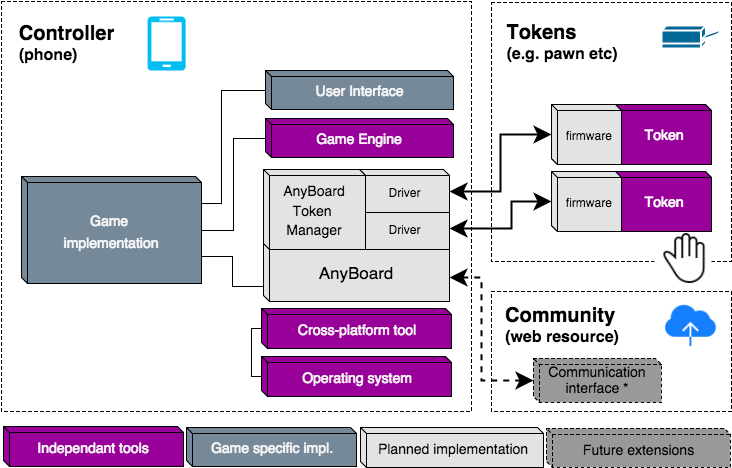
\includegraphics[width=12cm]{img/overview_architecture}
\centering
\caption{Architecture overview. AnyBoard will exist over three components. Tangible tokens such as digital pawns, a game controller/hub running on a smartphone, and an online application assisting the a community of both developers and players. My contribution in this thesis consists of the light grey boxes, denoted "Planned implementation".}
\label{fig:overview_architecture}
\end{figure}

\section{Phone-Token communication}
The means of communicating easily with different tokens is the most central component of AnyBoard. We aim for decoupled token-specific code, to address the requirements in table \ref{freq:token}.

TokenManager is a static component that handles the scanning and connecting/disconnect to tokens.
Its purpose is to identify nearby tokens, and determine an appropriate driver for the token to use. TokenManager has an own driver for this purpose. 

In figure \ref{fig:anypawn_architecture} we see this illustrated. Upon finding suitable drivers for detected tokens, TokenManager instantiates Token A1, Token A2 and Token B. These are Token Class instances, which – seen from the developers point of view – work as a sort of API on top of the tokens. These abstract away the low level communication and commands between AnyBoard and the specific tokens, and provide affordances such as ledOn(), ledOf() and print() functions.

\begin{figure}[ht]
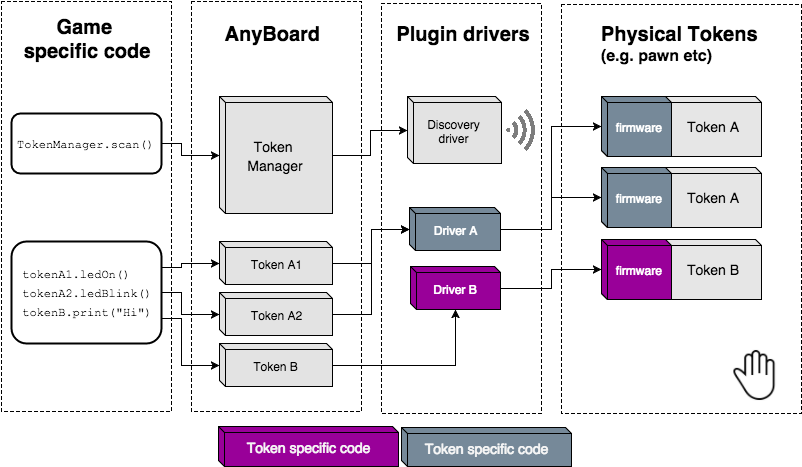
\includegraphics[width=12cm]{img/design_tokenmanager}
\centering
\caption{Communication overview between phone and token. An example where three tokens are discovered by the discovery driver and mapped to two different drivers, which handles the communication with their compatible tokens.}
\label{fig:anypawn_architecture}
\end{figure}


\section{Web-Phone communication}
Web is a component of AnyBoard that will not be implemented in this project, and will hence not be discussed or designed in any detail here. However, it's worth to note some thoughts about this important capability.

We imagine to use HTTP-communication where the phone sends requests to a API on the server. Suggested uses for this communication are:
\begin{enumerate}
\item Retrieving updated FAQ for the game.
\item Sending of events and actions in the game to enable multiplayer functionality, or viewers to watch a game.
\item Sending of events and actions in the game for history/logging.
\item Gathering statistics of usage.
\item Download new games from a Game store
\item Retrieve updates for a current games
\end{enumerate}

The basic tool necessary to enable this sort of communication is capability of communication over the HTTP-protocol. This capability could also be a useful feature for developers that wish to encapsulate web services into their board game or use physical devices that communicate using web APIs. 

This capability is already built into the JavaScript language, with the class XMLRequest. Abstracted HTTP calls using Ajax is also available in a variety of other JavaScript libraries. We therefore see no obstacles for this capability, even without designing for it in the current phase.